\chapter{Quantitative Description Of The Simulation And Reality}
For the evaluation of the effectivity of the containments strategy tested, it is necessary to make the simulation as realistic as possible. Still some assumptions will be made to keep the complexity and runtime reasonable. 
All statistics given here have been provided by Dr. Jörn Gethmann and Dr. Harald Lentz of the FLI for the sake of implementing the simulation. They have been extracted from HI Tier (Herkunftssicherungs- und Informationssystem für Tiere), a nation wide database database containing data about cattle in Germany. All cows need to be registered in this database as soon as they get an ear tag. Every trade needs to be announced here. This means every farmer has to register a cow that left his/her premise and the farmer on the receiving end need to input that he got the cow with the specified ear tag. Every death and every import or export needs to be tracked here as well.
\paragraph{Reliability Of The Data Provided By HI Tier}
According to \citep{personalCom} the data given by HI Tier is very reliable, since it has build in tests for the consistency of the data. For example a farm that did not notify the system that it bought a cow will not be able to tell the system that this cow died. On the other hand it could happen that the wrong ear tag number is put into the system or that farmers do not apply an ear tag before a calf dies, because they want to save money in case the calf dies early. Therefore some errors could occur and the statistics could be wrong.
\section{Breeding Dynamics}
The breeding dynamics are the foundation of a working simulation, because they lead to the demography that is necessary for the disease to spread properly, since the development of the disease within the body of a pregnant cow and it's calf is strongly influenced by the time window in which the infection takes place.
The breeding dynamics will be tested on a single farm since trading should have no effect on them\footnote{The single farm is put into a network with a slaughterhouse so that the farm can keep it's size stable by dumping all cows produced.}.
\paragraph{First Calving Time}
The time of the first calving is dependant on multiple distributions:
\begin{itemize}
\item age of first insemination
\item success rate of inseminations
\item rate of aborts
\item duration of pregnancy 
\item time before trying to inseminate a second (or third) time
\end{itemize}
All of these distributions are defined in {\tt Model\_Constants.h} and the distributions put into a random number generator from the gnu scientific library (gsl). All of these distributions have been gathered, but can not directly be observed using the data from HI Tier, which is why we can only compare the results for the first calving time from HIT to the results from our simulation.
The results of the given distributions are shown in plot \ref{fig:firstCalvingTime}. 
It can be seen, that the position of the maximum from the HIT database is met by the results of the simulation quite well. Furthermore the results show that the data in HIT is not completely correct since it contains calvings of cows with an age of $400\,\text{days}$ which is too little since the time of first insemination for most cow races lays between eight and ten months ($240-300\,\text{days}$) and the pregnancy lasts at least nine months ($270\,\text{days}$), making up for a total of at least $510\,\text{days}$. 
\begin{figure}[htbp]
\centering
\noindent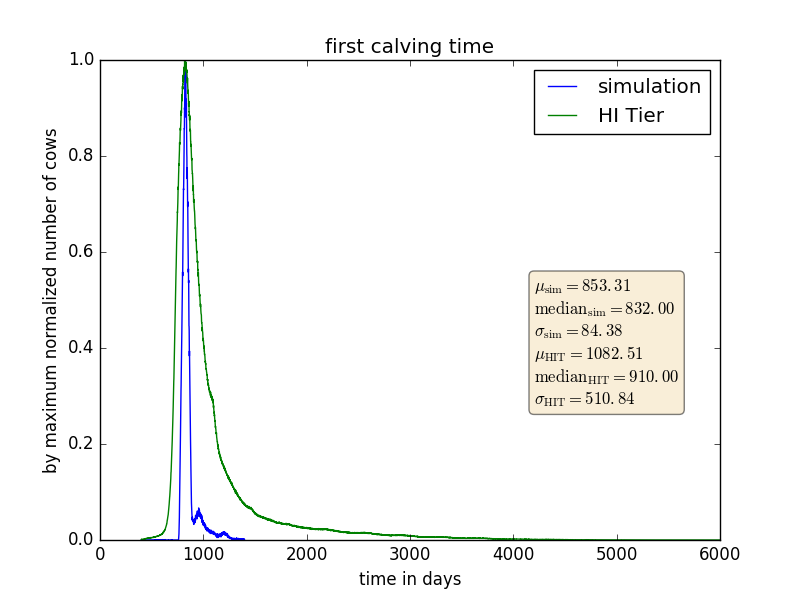
\includegraphics[width=0.8\linewidth,height=\textheight,
keepaspectratio]{firstCalvingTimesNormalwithCSV.png} 
\caption[First Calving Time]{The picture shows the first calving time of all cows in the simulation in comparison to the realistic data from HI Tier. Both have been normalized by the maximum number of cows with the given first calving time. The times in the yellow box are given in days.}
\label{fig:firstCalvingTime}
\end{figure}
On the right hand side of the peak the results from the simulation do not match reality all to well. This is mainly due to the fact that the simulation assumes a very simple model for the life cycle of a cow. In reality farmers will make their very individual decisions on when to inseminate their cows based on a lot of factors while the code just assumes that every cow will be inseminated right in the moment when it is possible. For farmers it should not make sense to inseminate a cow after 4 years of living but in reality it does make sense if a small farmer has little money and does not want to replace his cow (,he might even has feelings for). This could lead him to try more often to inseminate the same cow until it finally gets pregnant. 
Even though there is no full explanation for the mismatch on the right hand side of the peak, it can be seen that some features exist in the simulation which also exist in reality. There is a bump seen in the data from the HIT database around a time of $1100\,\text{days}$ which is supposedly caused by abortions. In principle it could also be caused by failed conceptions after an insemination, but the time between inseminations is usually less than a month so it can not account for a delay of roughly $270\,\text{days}$ in comparison to the peak at $827\,\text{days}$. 
A similar bump can be noticed in the data from the simulation. It is shifted a little bit to the left, so maybe the time of rest after an abortion is a little bit longer than it was foreseen by the distribution implemented in the code or the highest probability for an abortion is a little bit later. Another feature can be noticed in both: the data from HI Tier as well as the data from the simulation. Again the peak in the simulation data is shifted to the left and even further so than the first peak. This might have the same courses as for the first feature.
All in all it will be assumed that the simulation resembles reality sufficiently accurate. It can be seen that median and expectation value are higher in reality, which would lead to a higher probability for a cow to be infected before being inseminated successfully and therefore to recover and become immune before it finally reaches the state of pregnancy that makes the cow prone to give birth to a PI. Further research could analyze if this would have an impact on the disease dynamics such as the periodicity of outbreaks or the shares of the different compartments in the stable state. 
\paragraph{Intermediate Calving Time}
Just as the time of first calving is dependent on several distributions, the length of the time span between two calvings is also dependant on multiple distributions:
\begin{itemize}
\item time of rest after a calving before the first insemination,
\item probability of a successful insemination after the cow has been inseminated successfully before,
\item rate of an abortion,
\item duration of a pregnancy and
\item time before trying again to inseminate.
\end{itemize}
Picture \ref{fig:intermediateCalvingTime} shows the resulting distribution in the simulation and reality. Again it can be noted that the peaks of both distributions are very close to one another, even though the peak in the simulation is shifted by about $4\,\text{days}$. Compared to figure \ref{fig:firstCalvingTime} the variance in both distributions, but especially the data from the HIT database, is much lower. It shows that the approach of assuming that all farmers behave in the same way is much more realistic for the intermediate calving time then for the time of first calving.
\begin{figure}[htbp]
\centering
\noindent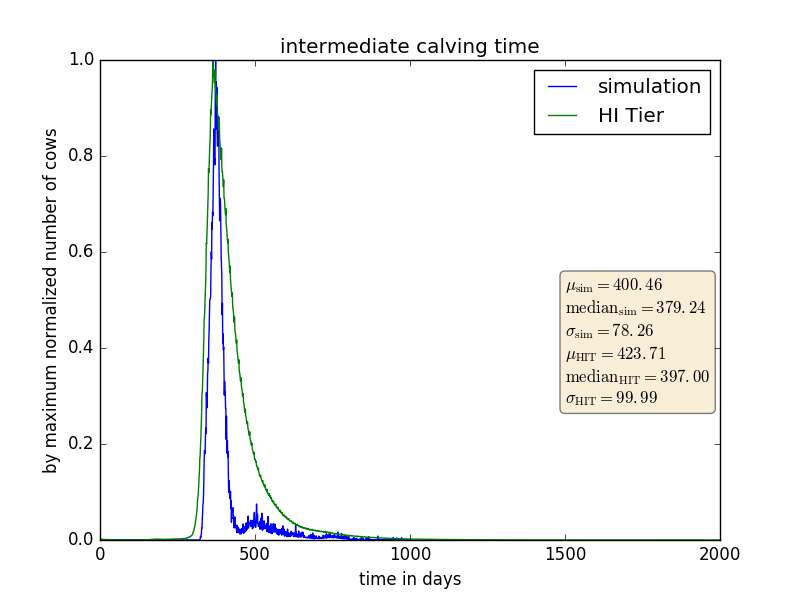
\includegraphics[width=0.8\linewidth,height=\textheight,
keepaspectratio]{intermediateCalvingTimeswithCSV.png} 
\caption[Intermediate Calving Times]{The length of the time between two calvings is shown by the graph. Both have been normalized by the maximum number of cows with the given first calving time. The times in the yellow box are given in days.}
\label{fig:intermediateCalvingTime}
\end{figure}
The data from HIT looks similar to a poisson distribution. The distribution's tails of both distributions are close to one another. The second feature of the simulation's data can only be explained by failed inseminations, because the difference between the two peaks is about $130\,\text{days}$, which can not be explained by failed pregnancies. Further side maxima can be observed between five and twenty five days before and after that feature. It is unclear why the slope between the first and second feature in the simulation is much steeper than the observed data from the HIT system. The later median and expectation value can lead to similar results in relation to the the disease dynamics as suggested for the first calving time above, but despite these differences the intermediate calving time is also considered to be sufficiently accurate. Also in this dataset absurd data points like intermediate calving times smaller than duration of pregnancy can be observed, which leads to the same conclusion. 

\section{Disease Dynamics}
To allow for a better understanding of the disease dynamics two simulations with a single farm each have been run. One of them had a herd size of about $400\cows$, while the other had a herd size of $40000\cows$. The latter is quite unrealistic, but still the difference in the herd size can lead to a better understanding of the way how the disease will behave. 
\begin{figure}[htbp]
\begin{minipage}{0.5\textwidth}
\centering
\noindent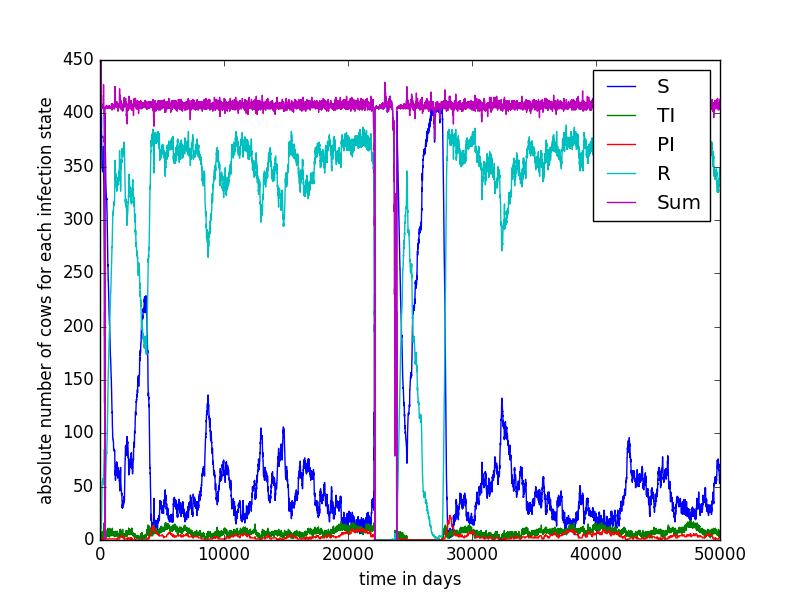
\includegraphics[width=0.9\linewidth,height=\textheight,
keepaspectratio]{totalEndemicNumbers300.png} 
\end{minipage}
\begin{minipage}{0.5\textwidth}
\centering
\noindent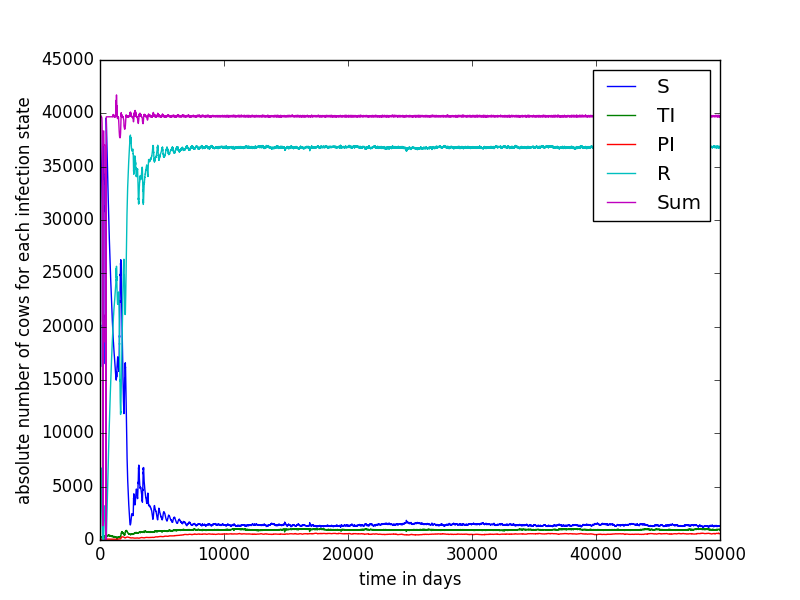
\includegraphics[width=0.9\linewidth,height=\textheight,
keepaspectratio]{totalEndemicNumbers40000.png} 
\end{minipage}
\caption[Absolute Numbers Of Compartments In Different Farm Sizes]{The plots show the absolute numbers of cows of the different compartments: (Susceptible $S$, Transiently Infected $TI$, Persistenly Infected $PI$, Recovered $R$ and the sum of all of them). Note that the compartment of recovered contains the animals protected by maternal antibodies too\protect\footnotemark. The left hand graph shows the behavior of a \glqq small\grqq\ farm with roughly $400\cows$ while the graph on the right hand side corresponds to the behaviour of a farm with approximately $40000\cows$.}
\label{fig:absoluteNumbersCompartmentsDifferentFarmSizes}
\end{figure} 
\footnotetext{It would also contain vaccinated animals, but there is no vaccination applied in the simulation which produced these datasets.}
The plots in figure \ref{fig:absoluteNumbersCompartmentsDifferentFarmSizes} show the different behavior of both farms in absolute numbers. Both plots show that the overall farm size is relatively stable. A stable state in terms of the disease spread is reached after less then $10000\days$ in the bigger farm, while the small farm remains relatively unstable. This is also due to the fact that the farm seems to be unable to keep it's size stable. This makes sense because small fluctuations in absolute values still make up for a big change in relative values. Some interesting characteristics shall be commented anyways. Both simulation runs and a number of other test runs have shown the same behavior in the beginning. They have been initialized with a percentage of recovered of $0\,\%$. The number of recovered rises while the number of susceptibles naturally declines. After some time (a few hundred to a few thousand days later) the number of recovered plummets while the number of susceptibles rises again just to fall back to it's stable state. This behavior, which resembles the aperiodic boundary case of the a critically damped oscillation, can be found in all simulations. The peculiar behaviour of the smaller farm during which it sells almost all of it's cows at some point in time can be found in almost every run with a single small farm. 
The figures \ref{fig:sharesCompartmentsDifferentFarmSizes} expose the fractions that the different compartments take up in regards to the total farm size. Both plots show that the distribution for a farm that had contact with a PI given in chapter \ref{chap:rlDataRegulationGermany}  can be met quite well. Since there is no evidence based data on the share of TIs on the whole population \citep{personalCom}, one has to compare the shares of recovereds and PIs. The share of recovered for the bigger farm oscillates around $92\,\%$ and the number of PIs oscillates between $1.3\,\%$ and $1.6\,\%$. The graphs that show the behavior of the smaller farm show a scenario which is more relevant for the simulation as a whole, since farms with a size of $40000\cows$ are not realistic at all. It can be seen that the seropositive population oscillates between $60\,\%$ and $95\,\%$, while the percentage of PIs oscillates between $0\,\%$ and about $6\,\%$. These fluctuations can be explained by the small system size and the resulting relatively big impact of a few animals. 

\begin{figure}[htbp]
\begin{minipage}{0.5\textwidth}
\centering
\noindent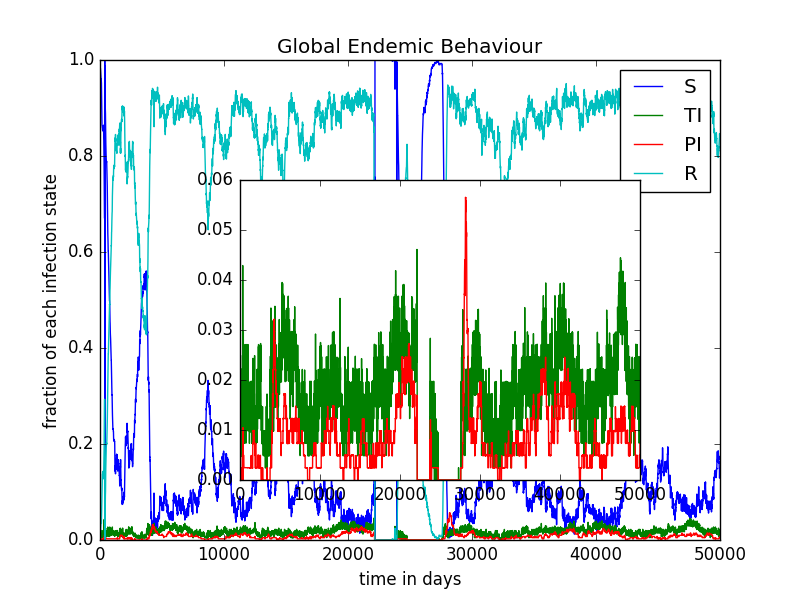
\includegraphics[width=0.9\linewidth,height=\textheight,
keepaspectratio]{endemicFractions300.png} 
\end{minipage}
\begin{minipage}{0.5\textwidth}
\centering
\noindent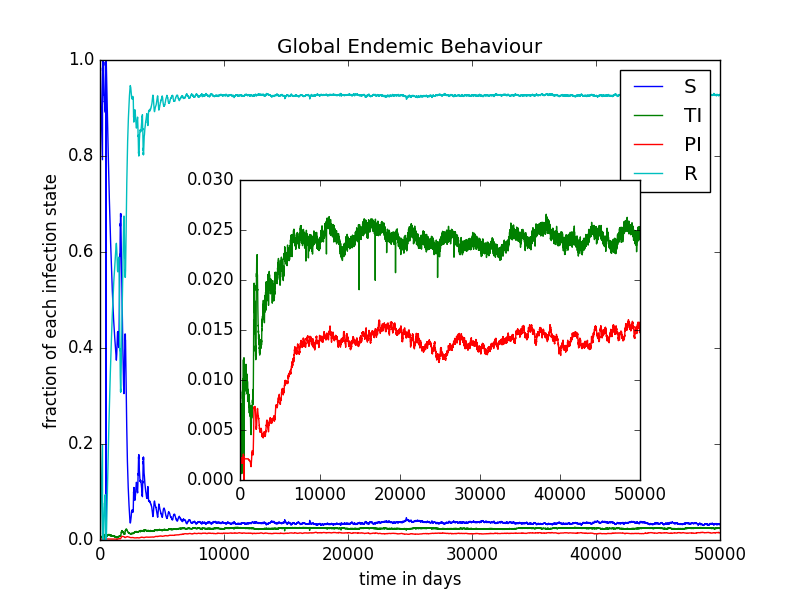
\includegraphics[width=0.9\linewidth,height=\textheight,
keepaspectratio]{endemicFractions40000.png} 
\end{minipage}
\caption[Shares Of Compartments In Different Farm Sizes]{The shown plots display the fractions of the different compartments (Susceptible $S$, Transiently Infected $TI$, Persistenly Infected $PI$ and Recovered $R$) in both examined farms (left: $N\approx 400\cows$, right: $N\approx 40000\cows$). Again the group of recovered individuals $R$ also contains those immune animals which are protected by maternal antibodies.}
\label{fig:sharesCompartmentsDifferentFarmSizes}
\end{figure} 

\section{Trading Dynamics} 
\section{Transients}